\section{Result}
Visualization of the clusters using Hierarchical clustering:

\begin{figure}[H]
    \centering
    \begin{subfigure}[b]{0.45\textwidth}
        \centering
        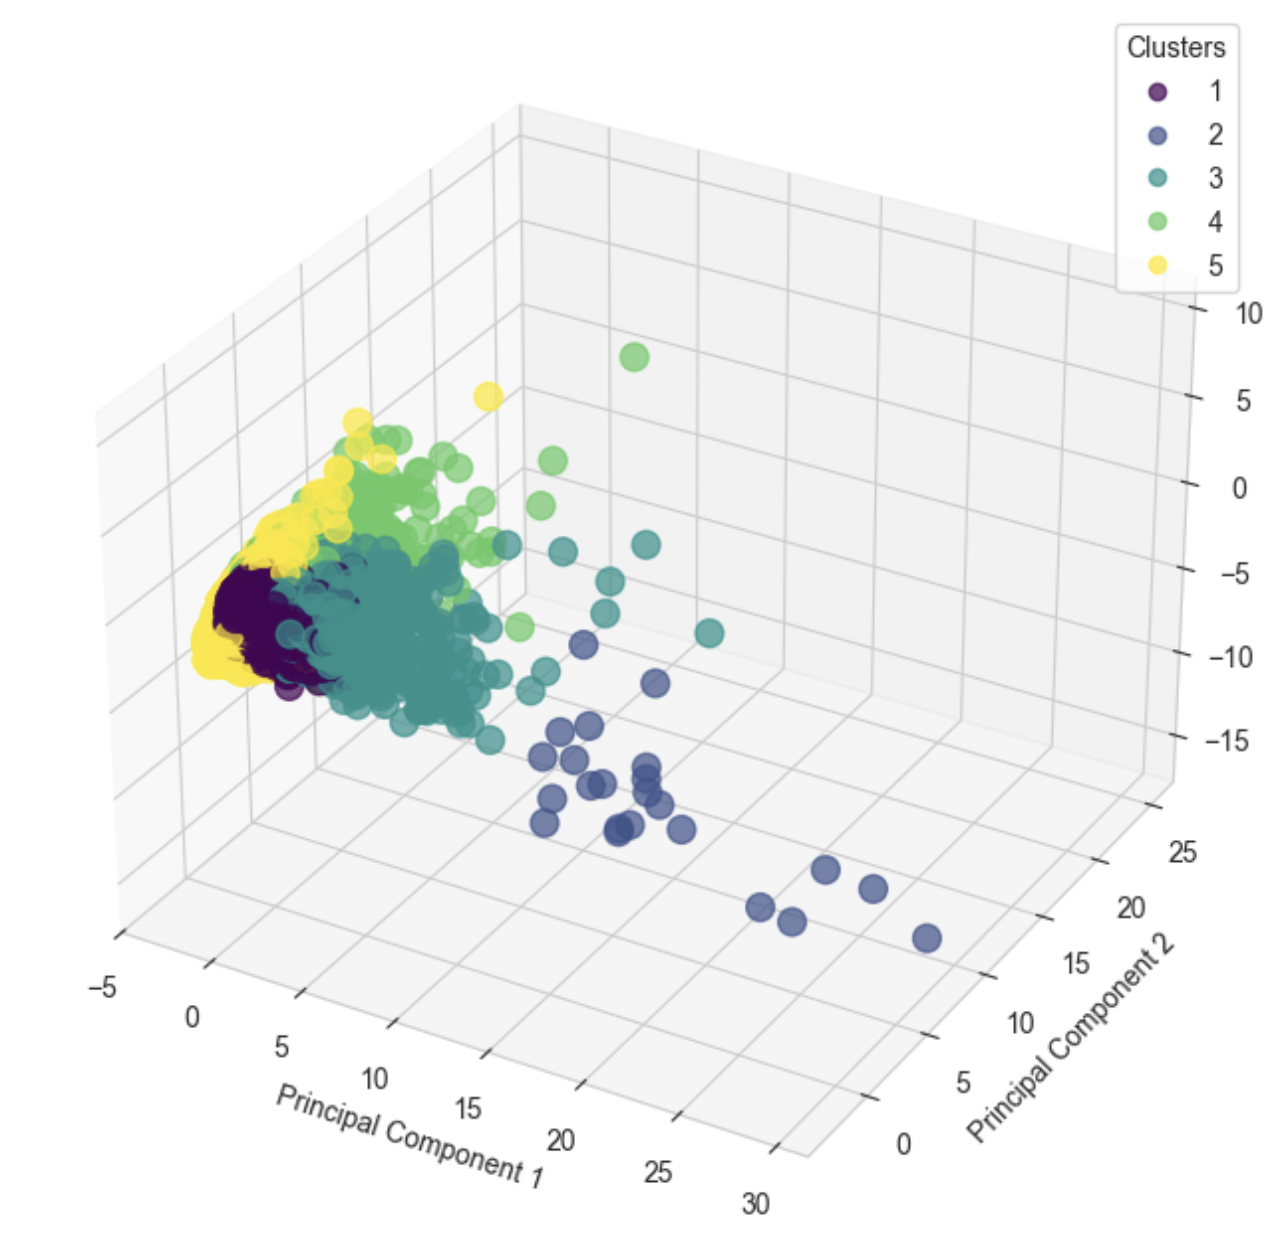
\includegraphics[width=\textwidth]{src/figs/3d_PCA_HC.png}
        \caption{3D PCA visualization of clusters}
        \label{fig:3D_pca}
    \end{subfigure}
    \hfill
    \begin{subfigure}[b]{0.45\textwidth}
        \centering
        \raisebox{0.3cm}{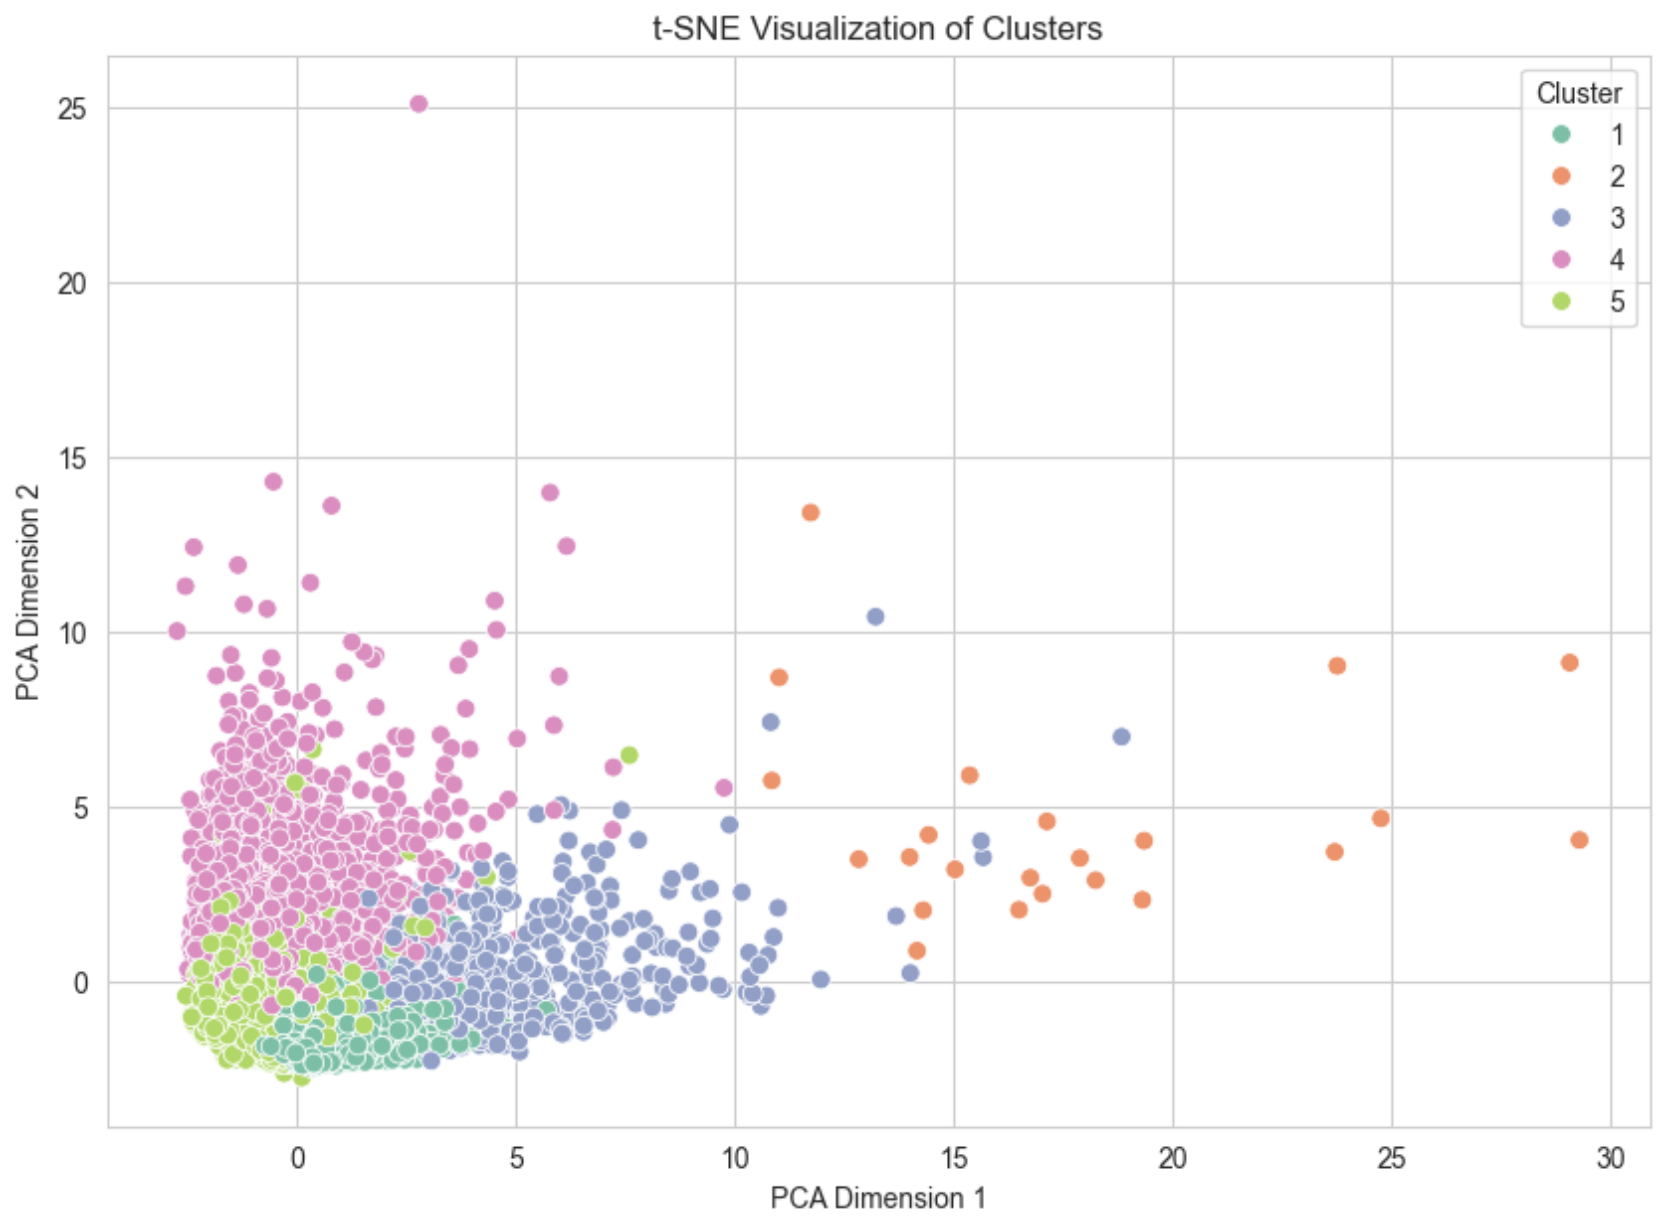
\includegraphics[width=\textwidth]{src/figs/2d_PCA_HC.png}} % Adjusts the image height
        \caption{2D PCA visualization of clusters}
        \label{fig:PCA_2d}
    \end{subfigure}
    \caption{Clustering visualizations: 3D (left) and 2D (right).}
    \label{fig:comparison1}
\end{figure}

\begin{figure}[H]
    \centering
    \begin{subfigure}[b]{0.45\textwidth}
        \centering
        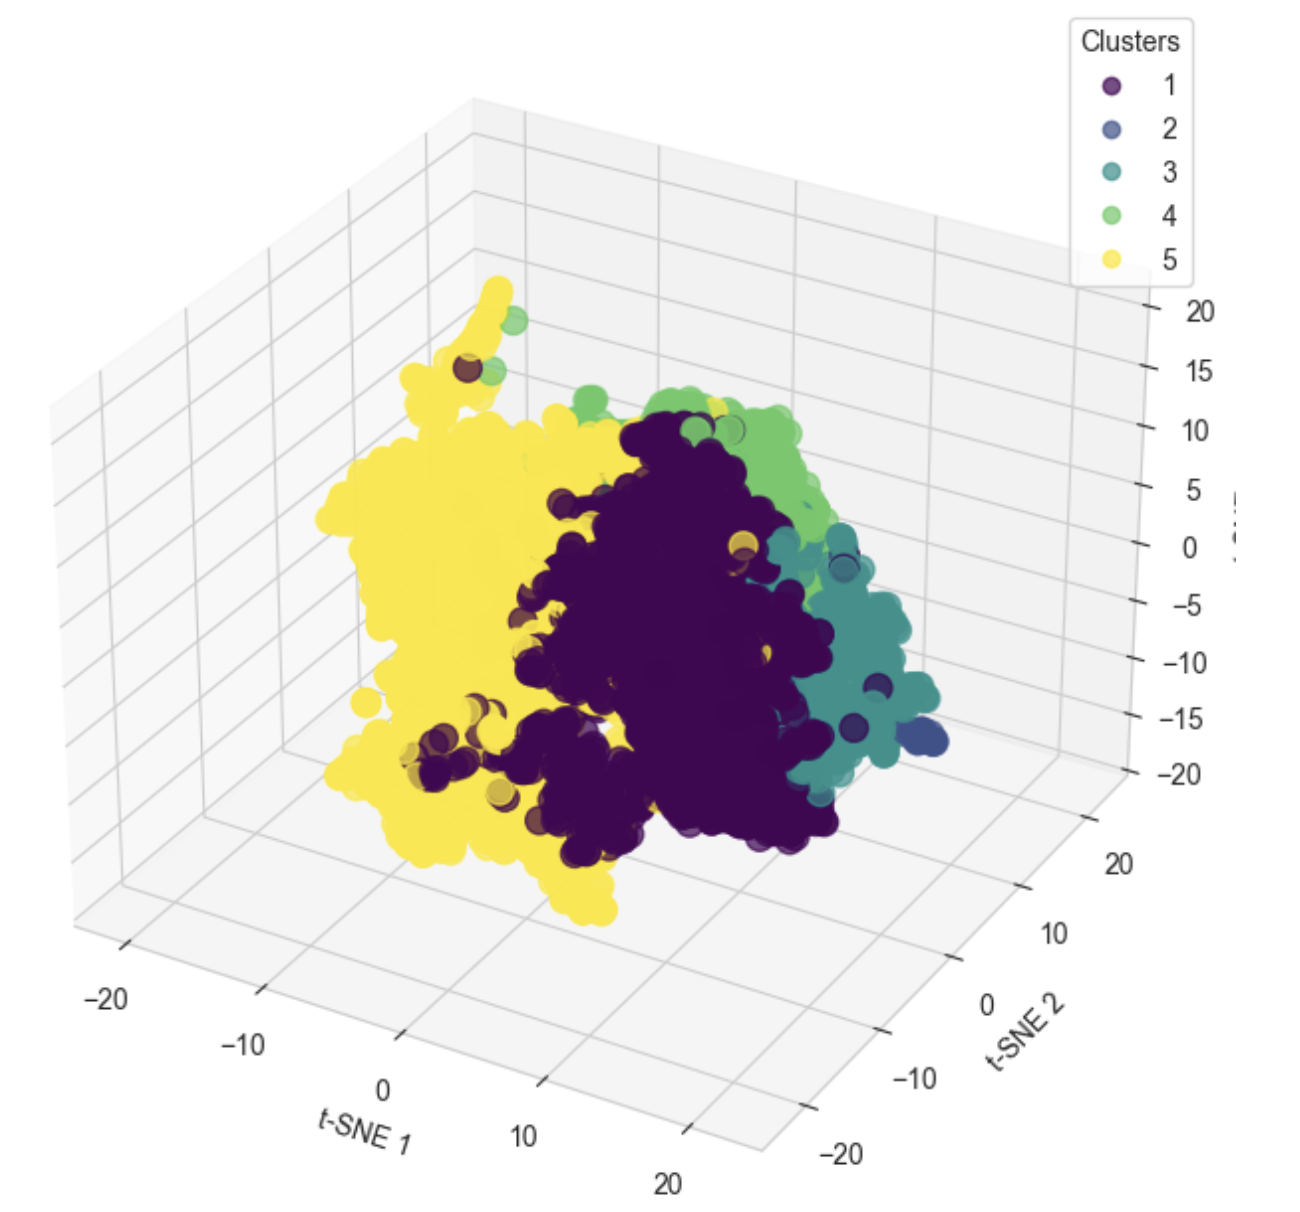
\includegraphics[width=\textwidth]{src/figs/3d_t-SNE.png}
        \caption{3D t-SNE visualization of clusters}
        \label{fig:3D_tsne}
    \end{subfigure}
    \hfill
    \begin{subfigure}[b]{0.45\textwidth}
        \centering
        \raisebox{0.3cm}{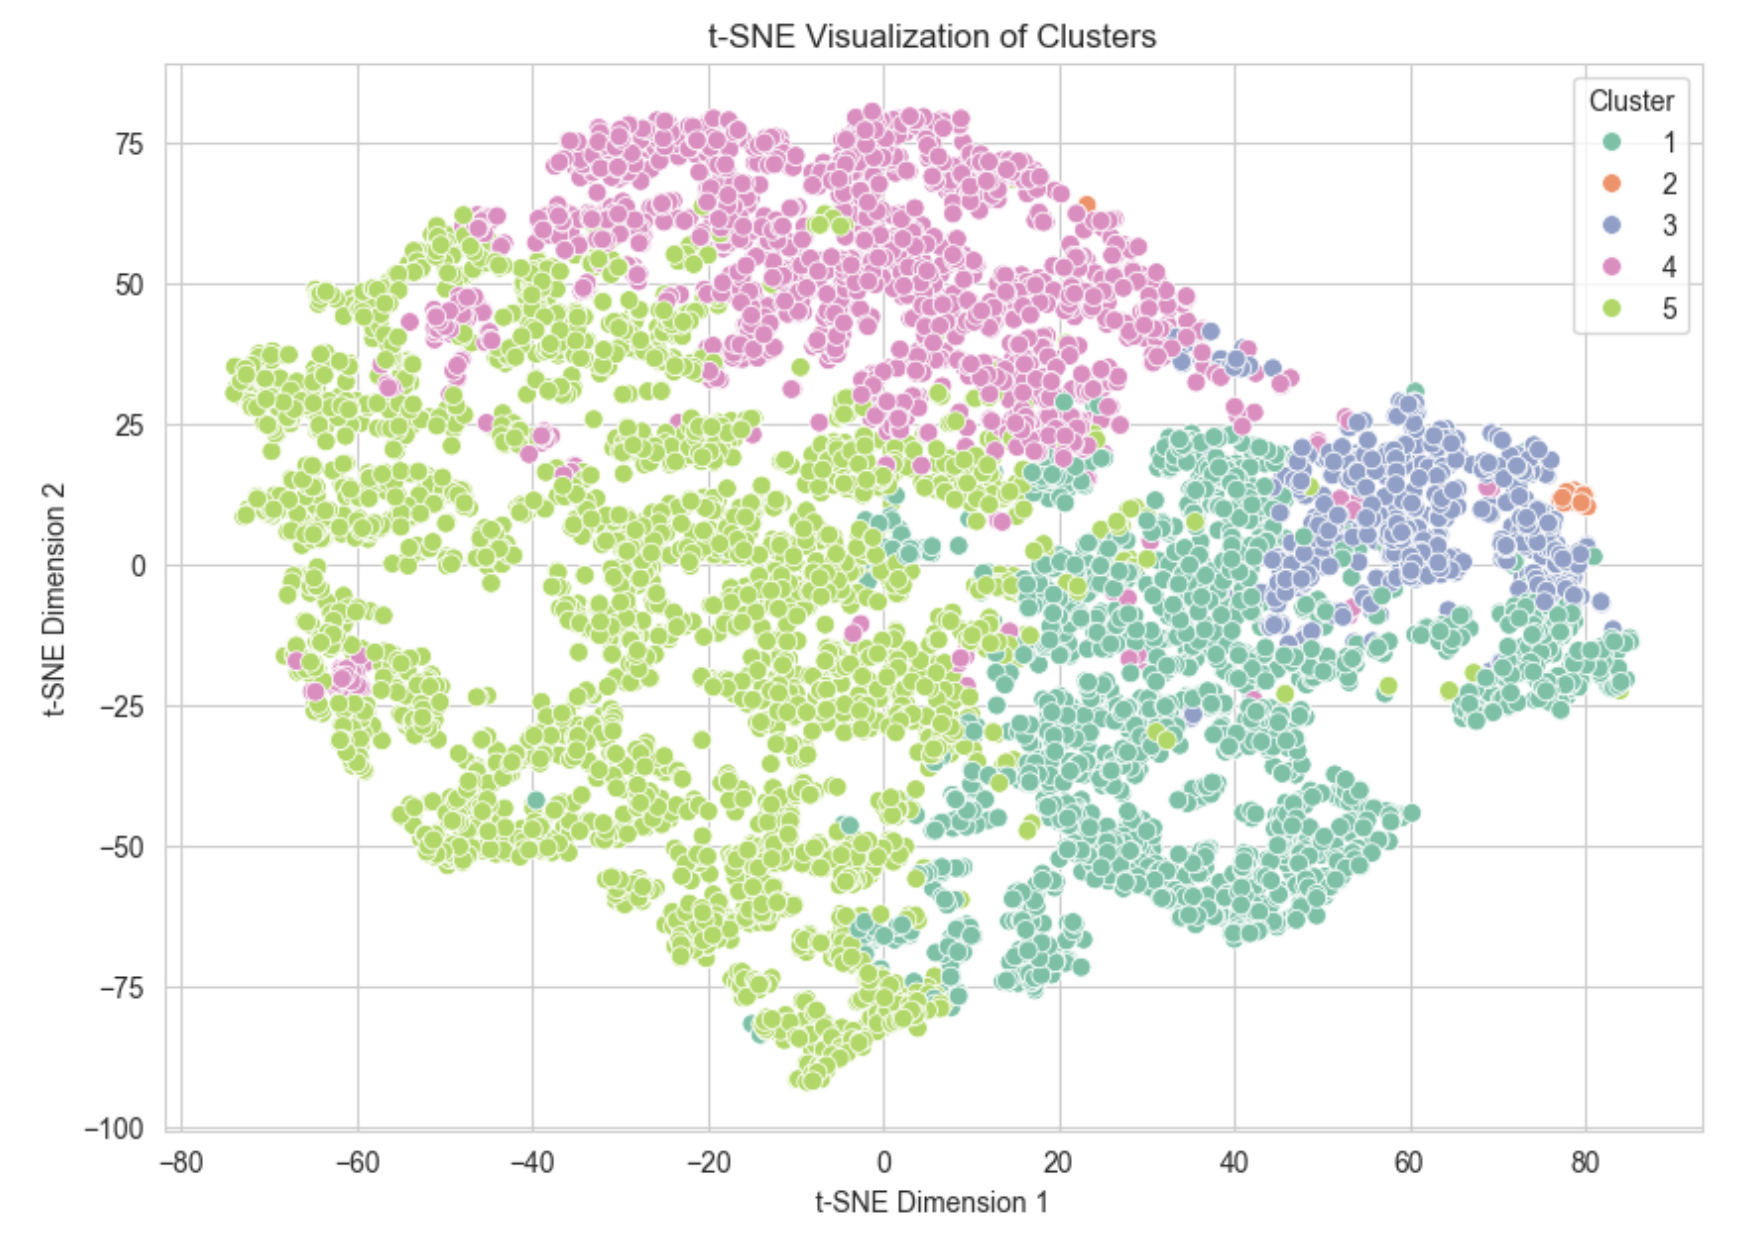
\includegraphics[width=\textwidth]{src/figs/2d_t-SNE.png}} % Adjusts the image height
        \caption{2D t-SNE visualization of clusters}
        \label{fig:2D_tsne}
    \end{subfigure}
    \caption{Clustering visualizations: 3D (left) and 2D (right).}
    \label{fig:comparison2}
\end{figure}